\documentclass[11pt]{article}
\usepackage[utf8]{inputenc}
\usepackage{polski}
\usepackage{graphicx}
\usepackage{array}
\usepackage{paralist}
\usepackage{verbatim}
\usepackage{subfig}
\usepackage{amsmath}
\usepackage{float}
\usepackage{amsthm}
\usepackage{amssymb}
\usepackage{pdfpages}
\usepackage{amsfonts}
\usepackage{tikz}
\usepackage{wasysym}
\usepackage[linguistics]{forest}
\usetikzlibrary{shapes,backgrounds}
\usepackage[margin=1in]{geometry}
\setlength\parindent{0pt}
\theoremstyle{definition}
\newtheorem{zadanie}{Zadanie}
\numberwithin{zadanie}{subsection}
\renewcommand*{\proofname}{Rozwiązanie}
\newtheorem{theorem}{Twierdzenie}
\title{Matematyka dyskretna}
\author{Igor Nowicki}
\begin{document}
\maketitle
\tableofcontents

\section{Cheat sheet}

Rzeczy na pierwsze kolokwium:
\begin{itemize}
    \item Relacje. Symetryczność, zwrotność, przechodniość. Macierz relacji, liczba możliwych relacji, klasy abstrakcji.
    \item Funkcje. Surjekcja, injekcja, bijekcja.
    \item Permutacje. Cykle rozłączne, inwersje, typ, znak.
    \item Zasada włączania-wyłączania zbiorów.
    \item Kombinacje zbiorów nieuporządkowanych.
    \item Zliczanie kombinacji ustawień elementów rozróżnialnych, nierozróżnialnych.
    \item Rozmieszczenia uporządkowane.
    \item Wektory charakterystyczne, zbiór potęgowy.
    \item Zliczanie całkowitych rozwiązań równań i nierówności.
    \item Zliczanie najkrótszych dróg na kracie z warunkami.
    \item Zasada Dirichleta.
    \item Zbiory z powtórzeniami, funkcje tworzące.
\end{itemize}

\subsection{Relacje}

Najprościej - relacja jest procesem powiązania pary elementów z jednego zbioru w parę uporządkowaną. Dla relacji mamy wyszczególnione trzy przypadki szczególne:
\begin{itemize}
    \item relacja jest \textit{symetryczna}, jeśli $xRy \Rightarrow yRx$. Odpowiada to symetryczności macierzy relacji.
    \item relacja jest \textit{zwrotna}, jeśli dla każdego $x\in X$ mamy $xRx$. Odpowiada to jedynkowej diagonali macierzy relacji.
    \item relacja jest \textit{przechodnia}, jeśli $xRy$ oraz $yRz$ implikują $xRz$.
\end{itemize}

Przy spełnieniu tych trzech warunków możemy mówić o \textit{relacji równoważności}. Podzbiór $X$ dla którego $R$ jest relacją równoważności nazywany jest \textit{klasą abstrakcji}.

\subsection{Funkcje}

Funkcja jest procesem powiązania pary elementów z dwóch zbiorów (\textit{dziedziny} i \textit{przeciwdziedziny}) w parę, z założeniem że każdy element dziedziny ma przyporządkowany dokładnie jeden element z przeciwdziedziny. Wyszczególniamy trzy przypadki szczególne funkcji:

\begin{itemize}
    \item funkcja jest \textit{injektywna} (różnowartościowa) - każdy element $x\in X$ ma przyporządkowany inny element $y\in Y$. Jest to oczywiście możliwe, gdy $|X|\leq|Y|$.
    \item funkcja jest \textit{surjektywna} (na) - każdy element $y\in Y$ jest przyporządkowany przynajmniej jednemu elementowi $x\in X$. Jest to możliwe gdy $|X|\geq|Y|$.
    \item funkcja jest \textit{bijektywna} - spełnione są jednocześnie warunki iniekcji i surjekcji, wszystkie $x\in X$ oraz $y\in Y$ są ze sobą powiązane w pary. Oznacza to, że $|X|=|Y|$.
\end{itemize}

\subsection{Permutacje}

Permutacją $\pi$ można określić dowolne przyporządkowanie różnowartościowe ze zbioru $\{1,...,n\}$ do zbioru $\{1,...,n\}$. Oznacza to, że możliwych permutacji dla $n$-elementowego zbioru jest zawsze $n!$.

Przy permutacjach mamy parę pojęć, które dobrze jest mieć zapisane z boku:

\begin{itemize}
    \item cykl rozłączny - dla danego $x\in X$ najmniejszy taki ciąg gdzie $\{x, \pi(x), \pi^2(x),...,\pi^{r}(x)\}$, oraz $\pi^{r+1}(x) = x$.
    \item inwersja - para liczb $a_j, a_k$, gdzie $j<k$ oraz $a_j > a_k$ (czyli para wartości większa-mniejsza w ciągu).
    \item typ permutacji - zapis polegający na przedstawieniu ile występuje $k$-elementowych cykli w $n$-elementowej permutacji. Możemy to zapisać za pomocą iloczynu $1^{\alpha_1}2^{\alpha_2}...n^{\alpha_n}$, lub za pomocą wektora $(\alpha_1,\alpha_2,...\alpha_n)$.
    \item znak permutacji - iloczyn znaków poszczególnych cykli w permutacji (wartości $\pm 1$), gdzie cykl o parzystej liczbie elementów jest \textbf{nieparzysty} (wartość $-1$), natomiast cykl o nieparzystej liczbie elementów jest \textbf{parzysty}.
\end{itemize}

\subsection{Zasada włączania-wyłączania zbiorów}

\begin{figure}[H]
    \centering
    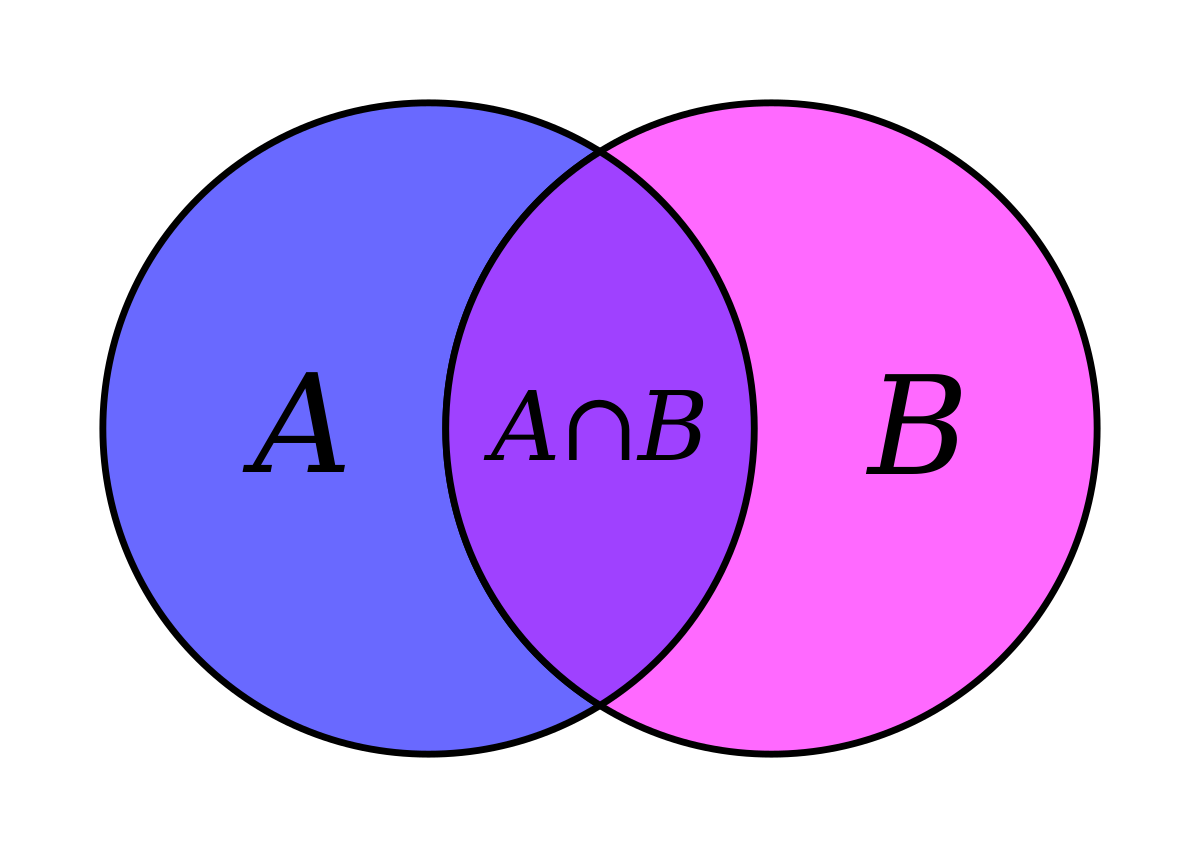
\includegraphics[width=0.3\linewidth]{ex-in-2.png}
\end{figure}

Najprościej - załóżmy że chcemy policzyć moc (lub miarę) sumy zbiorów $A\cup B$, jednak wiemy również, że istnieje jakieś przecięcie tychże zbiorów $A\cap B$. Wzór który możemy zastosować to:

$$|A\cup B| = |A|+|B| - |A\cap B|.$$

\begin{figure}[H]
    \centering
    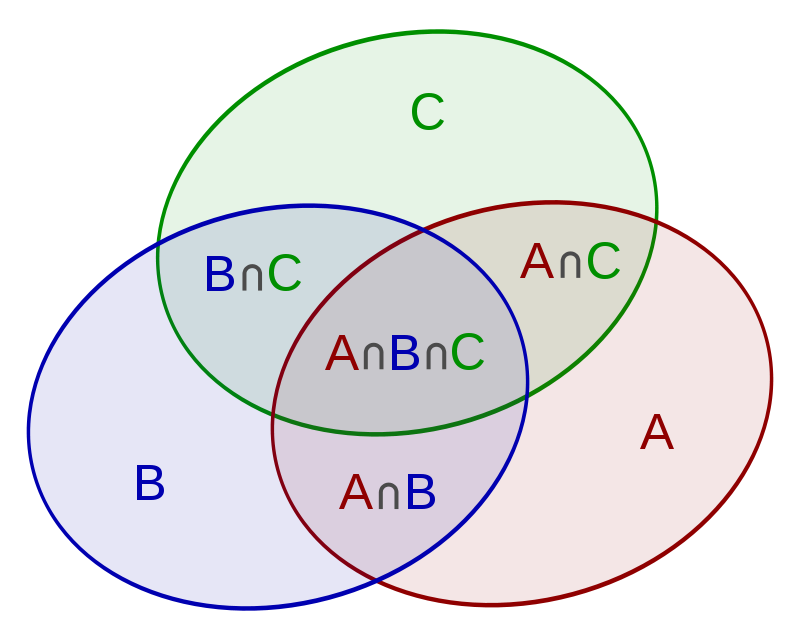
\includegraphics[width=0.3\linewidth]{in-ex.png}
\end{figure}

Dalej - dla zbiorów trójelementowych analogiczną sumę możemy wyznaczyć jako:

$$|A\cup B\cup C| = |A|+|B|+|C| - |A\cap B| - |A\cap C| - |B\cap C| + |A\cap B\cap C|.$$


W ogólności wzór przedstawia się następująco:

$$\left|\bigcup_{i=1}^n A_i\right| = \sum_{i=1}^n\left|A_i\right|-\sum_{i,j:\,i<j}\left|A_i\cap A_j\right| + \sum_{i,j,k:\,i<j<k}\left|A_i\cap A_j\cap A_k\right|-\ \dots + (-1)^{n-1} \left|A_1\cap\cdots\cap A_n\right|.$$
\subsection{Kombinacje zbiorów nieuporządkowanych}

Załóżmy że chcemy włożyć $n$ nierozróżnialnych piłek do $m$ rozróżnialnych pudełek - na ile sposobów można to zrobić? Otóż każda piłka ma przyporządkowane jedno i tylko jedno pudełko do którego należy - rozwiązaniem będzie $m^n$.

\subsection{Zliczanie kombinacji ustawień elementów rozróżnialnych, nierozróżnialnych}

Załóżmy że chcemy ustawić $n$ piłek w $m$ slotach, gdzie $n\geq m$ - na ile sposobów możemy to zrobić? Otóż będzie tu się stosował symbol Newtona, tj. $\binom m n = \frac{m!}{n!(m-n)!}$, dla nierozróżnialnych piłek, oraz $\binom m n\cdot n!$ dla rozróżnialnych piłek.

\subsection{Rozmieszczenia uporządkowane}

Chcemy poustawiać $n$ klientów w $m$ kolejkach, gdzie kolejność klientów ma znaczenie - na ile sposobów możemy to zrobić? Stosuje się wzór $n^{\overline{m}} = n\cdot(n+1)\cdot...\cdot(n+m-1)$.

\subsection{Wektory charakterystyczne, zbiór potęgowy}

Mając zbiór $n$ elementów (załóżmy że możemy wprowadzić jakąś kolejność dla tych elementów) możemy każdemu z podzbiorów przyporządkować \textbf{wektor charakterystyczny} - ciąg zer i jedynek określających który z elementów zbioru się pojawia, a który nie. Pytając o moc zbioru potęgowego, czyli liczbę wszystkich możliwych podzbiorów, docieramy w ten sposób do analogii z liczbą wszystkich możliwych liczb binarnych o $n$ bitach: $2^n$.

\subsection{Zliczanie najkrótszych dróg na kracie z warunkami}


\begin{center}
    \begin{tabular}{ |c|c|c|c|c|c|c|c|c|c| }
        \hline
         &  &  &  &  &  &  &  &  & \\
        \hline
         &  &  &  &  &  &  &  &  & \\
        \hline
         &  &  &  &  &  &  &  &  & \\
        \hline
         &  &  &  &  &  &  &  &  & \\
        \hline
    \end{tabular}
\end{center}

Mając kratę $n\times m$ i poszukując wszystkich możliwych dróg z lewego dolnego rogu do prawego górnego możemy rozwiązać równanie w następujący sposób - musimy wykonać $n+m$ kroków, oraz $n$ z nich musi być w prawo (bądź, alternatywnie, $m$ z nich musi być do góry). Znalezienie liczby możliwych najkrótszych dróg (o $n+m$ krokach) sprowadza się do policzenia wszystkich kombinacji rozmieszczenia $n$ (lub $m$) strzałek w $n+m$ slotach: $\binom{n+m}{n}=\binom{n+m}{m}=\frac{(n+m)!}{n!m!}$.

\subsection{Zliczanie całkowitych rozwiązań równań i nierówności}

Mając zadanie policzenia wszystkich możliwych rozwiązań całkowitoliczbowych równania:

$$x_1+x_2+...+x_m = n,$$

gdzie $x_i\geq 0$, możemy sprowadzić do do poruszania się po kracie (patrz poprzedni paragraf) o $m$ węzłach w jednej osi (czyli $m-1$ krokach) oraz $n$ węzłach w drugiej. Liczba możliwych rozwiązań zatem to $\binom{n+m-1}{m-1}$.

Jeśli któraś z wartości stanowiłaby inną nierówność, należy dokonać podstawienia, tak by nowy zbiór zmiennych sprowadzał się do $x_i\geq 0$. Jeśli zamiast równania mamy nierówność, należy zsumować liczby wszystkich przypadków dla poszczególnych $n$.

\subsection{Zasada Dirichleta}

Mamy $n$ skarpet w $m$ szufladach, gdzie $n > r*m$ - należy udowodnić, że istnieje szuflada w której jest ponad $r$ skarpet. Korzystamy z zasady Dirichleta, tzn. założenia że jeśli $r$ jest maksymalną wartością elementów w $m$ pudełkach, to nie może ich być więcej niż $m\cdot r$. Zatem jeśli elementów jest więcej niż $m\cdot r$, oznacza to że istnieje szuflada w której jest przynajmniej $r+1$ elementów.

\subsection{Zbiory z powtórzeniami, funkcje tworzące}

Definiowany jest szczególny typ zbioru, \textit{zbiór z powtórzeniami} - przykładowo, $\{3a,2b,4c\}$. Zadajemy teraz pytanie, ile jest takich podzbiorów że liczba $a$ jest parzysta, liczba $b$ nieparzysta etc. Pewną metodą rozwiązania jest użycie \textit{funkcji tworzącej} - iloczynu wielomianów odpowiadających $a, b, c$ w których każda potęga odpowiada konkretnej liczbie elementów. I tak, warunek parzystego $a$, nieparzystego $b$ oraz parzystego $c$ można przetłumaczyć na:

$$(x^0+x^2)(x^1)(x^0+x^2+x^4) = x^0+x^3+x^5+x^7,$$

czyli zbiorów zero-elementowych będzie dokładnie 1, zbiorów 1-elementowych: 0,
zbiorów 2-elementowych: 0, zbiorów 3-elementowych: 1, i tak dalej.

\section{Rozwiazania zadań}
\subsection{Relacje}
\begin{zadanie}
    Dana jest relacja $R$ na zbiorze $X = \{a,b,c,d,e,f\}$, reprezentowana macierzą $\mathcal M$:

    $$\mathcal M = \begin{pmatrix}
            1 & 0 & 1 & 0 & 0 & 0 \\
            0 & 1 & 0 & 0 & 0 & 0 \\
            0 & 0 & 1 & 0 & 0 & 0 \\
            0 & 0 & 0 & 1 & 0 & 0 \\
            0 & 1 & 0 & 0 & 1 & 0 \\
            0 & 0 & 1 & 0 & 0 & 1
        \end{pmatrix}$$

    \begin{enumerate}[a)]
        \item Narysuj graf relacji $R$.
        \item W macierzy dodaj jak najmniej jedynek by powstała macierz określająca relację równoważności $R'$.
        \item Wyznacz klasy abstrakcji relacji $R'$.
    \end{enumerate}
\end{zadanie}
\begin{proof}
    \begin{enumerate}[a)]
        \item Graf relacji $R$ polega na graficznym przedstawieniu relacji pomiędzy punktami.

              % Tutaj widzimy, że mamy następujące połączenia:
              %       \begin{itemize}
              %           \item z $a$ do $a$,
              %           \item z $a$ do $c$,
              %           \item z $b$ do $b$,
              %           \item z $c$ do $c$,
              %           \item z $d$ do $d$,
              %           \item z $e$ do $b$,
              %           \item z $e$ do $e$,
              %           \item z $f$ do $c$,
              %           \item z $f$ do $f$.
              %       \end{itemize}

              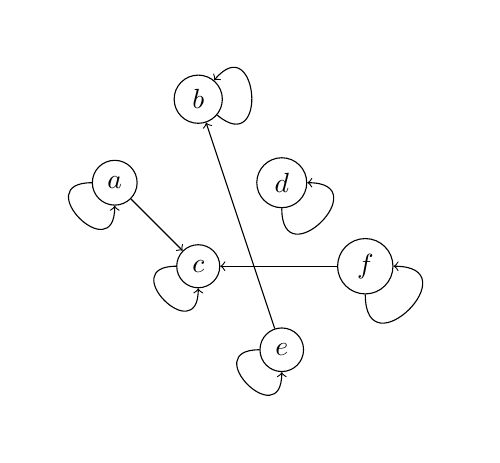
\begin{tikzpicture}[main/.style = {draw, circle}, node distance={15 mm}]
                  \node[main] (a) {$a$};
                  \node[main] (b) [above right of=a] {$b$};
                  \node[main] (c) [below right of=a] {$c$};
                  \node[main] (d) [above right of=c] {$d$};
                  \node[main] (e) [below right of=c] {$e$};
                  \node[main] (f) [above right of=e] {$f$};
                  \draw[->] (a) to [out=180,in=270,looseness=5] (a);
                  \draw[->] (a) -- (c);
                  \draw[->] (b) to [out=320,in=50,looseness=5] (b);
                  \draw[->] (c) to [out=180,in=270,looseness=5] (c);
                  \draw[->] (d) to [out=270,in=360,looseness=5] (d);
                  \draw[->] (e) -- (b);
                  \draw[->] (e) to [out=180,in=270,looseness=5] (e);
                  \draw[->] (f) -- (c);
                  \draw[->] (f) to [out=270,in=360,looseness=5] (f);
              \end{tikzpicture}


        \item Jeśli chcemy mieć relację równoważności, to musimy mieć spełnione następujące warunki:
              \begin{itemize}
                  \item relacja musi być zwrotna.
                        Warunek zwrotności jest spełniony, ponieważ dla każdego elementu $x\in X$ mamy $xRx$.
                  \item relacja musi być symetryczna,
                        Warunek symetrii można zapisać jako warunek tego by reprezentacja macierzowa $\mathcal M$ była symetryczna - brakuje nam wtedy zatem trzech jedynek do spełnienia ($\mathcal M_{ca}, \mathcal M_{be}, \mathcal M_{cf}$).
                  \item relacja musi być przechodnia,
                        Warunek przechodniości jest rozumiany jako "dla dowolnych $x,y,z\in X$, jeśli $x R y$ oraz $y R z$ to $x R z$".
              \end{itemize}
    \end{enumerate}

    Moglibyśmy również przedstawić relację równoważności jako warunek by wszystkie pola macierzy były jedynkowe.
\end{proof}

\begin{zadanie}
    Ile jest wszystkich relacji symetrycznych w zbiorze 6-elementowym?
\end{zadanie}
\begin{proof}
    \textbf{Relacją symetryczną} nazywamy taką relację $f$, że spełniony jest następujący warunek:

    $$\forall x,y\in A: x f y \Rightarrow y f x,$$

    tzn. jeśli $x$ jest w relacji $f$ z $y$, to $y$ jest w relacji $f$ z $x$.

    Zadanie możemy rozwiązać poprzez reprezentację relacji jako macierzy binarnej $n\times n$, gdzie $n$ jest liczbą elementów w zbiorze:

    \begin{align*}
         &
        \begin{matrix}
            a & b & c & d & e & f
        \end{matrix}    \\
        \begin{matrix}
            a \\b\\c\\d\\e\\f
        \end{matrix}
        \quad
         & \begin{bmatrix}
            0 & 0 & 0 & 0 & 0 & 0 \\
            0 & 0 & 0 & 0 & 0 & 0 \\
            0 & 0 & 0 & 0 & 0 & 0 \\
            0 & 0 & 0 & 0 & 0 & 0 \\
            0 & 0 & 0 & 0 & 0 & 0 \\
            0 & 0 & 0 & 0 & 0 & 0
        \end{bmatrix}
    \end{align*}
    gdzie $0$ oznacza brak relacji, natomiast $1$ oznacza istniejącą relację wartości z kolumny i wartości z wiersza (w tej kolejności). Od razu widać, że dla relacji symetrycznej wyżej przedstawiona macierz musi być symetryczna - tj. warunek $xfy\Rightarrow yfx$ tłumaczy się jako warunek $a_{ij} = a_{ji}$ w języku macierzy. W takiej sytuacji mamy tak naprawdę $n\cdot(n+1)/2$ wartości którymi możemy manipulować. Ponieważ dozwolone wartości są $0$ lub $1$, oznacza to $2^{n\cdot(n+1)/2}$ możliwych relacji - dla $n = 6$ mamy $2^{3\cdot7} = 2,097,152$ relacji.
\end{proof}

\begin{zadanie}
    Zbiór $X=\{a,b,c,d,e,f,g,h,i,j,k\}$ rozbito na podzbiory $A=\{a,c,d\}$, $B=\{e,h,i,j\}$, $C=\{b,k\}$, $D=\{f,g\}$.

    \begin{enumerate}[a)]
        \item Zdefiniuj w X relację równoważności R taką, by podane zbiory były klasami abstrakcji relacji R. Ile różnych relacji równoważności o powyższej własności można zdefiniować?
        \item Ile zer ma macierz binarna relacji z podpunktu a)?
    \end{enumerate}
\end{zadanie}
\begin{proof}
    \begin{enumerate}[a)]
        \item Klasa równoważności może być reprezentowana jako macierz relacji wypełniona jedynkami. Ponieważ wszystkie elementy ze zbioru $X$ są w jednej z klas równoważności, nie mamy żadnych stopni swobody - jest tylko jedna relacja którą możemy zdefiniować dla tak zadanych warunków.
        \item Cała macierz relacji ma $11^2=121$ elementów. Każdy z podzbiorów jest reprezentowany jako macierz jedynek - w sumie jest to $3^2+4^2+2^2+2^2 = 9+16+4+4=33$ elementy. Zatem mamy $121-33 = 88$ zer.
    \end{enumerate}
\end{proof}
\begin{zadanie}
    $A = \{1,2,3,B,\{1,2\}\}; B = \{1,2,A,\{1,2\},x,y,z\}.$ Ile jest:

    \begin{enumerate}[a)]
        \item funkcji $f: A\times B\to A$?
        \item funkcji różnowartościowych $g: B\to A$?
        \item funkcji różnowartościowych $g: B\to A\times B$.
        \item surjekcji $s:A\to B$
        \item podzbiorów zbioru $B\times A$?
        \item wszystkich relacji w zbiorze A?
        \item Ile jest relacji symetrycznych w B?
        \item Ile jest relacji zwrotnych w B?
    \end{enumerate}

\end{zadanie}
\begin{proof}
    \begin{enumerate}[a)]
        \item Zliczamy na ile sposobów można przyporządkować elementy z dziedziny $A\times B$ ($|A\times B|=5\cdot7=35$ elementów) do elementów z przeciwdziedziny $A$ ($|A|=5$). Każda wartość dziedziny może mieć jeden i tylko jeden element z przeciwdziedziny - zatem liczba rozwiązań to $5^{35}$.
        \item Funkcja różnowartościowa polega na warunku pojawiania się co najwyżej raz elementów z przeciwdziedziny - tj. $f(x_1) = f(x_2)\implies x_1=x_2$. Ponieważ w $B$ mamy 7 elementów, a w $A$ mamy 5 elementów, to niemożliwe jest takie przyporządkowanie, by każdy element dziedziny miał unikalny odpowiadający mu element przeciwdziedziny.
        \item Przyporządkowujemy z dziedziny 7 elementów do przeciwdziedziny 35 elementów w sposób różnowartościowy. Wynikiem będzie $35\cdot34\cdot...\cdot29$ możliwości.
        \item Surjekcja polega na zaalokowaniu wszystkich elementów przeciwdziedziny - czyli każda wartość z B powinna się pojawić przynajmniej raz. Ponieważ elementów zbioru $A$ jest mniej niż elementów zbioru $B$, taka sytuacja jest niemożliwa.
        \item Moc zbioru potęgowego zbioru 35 elementów to $2^{35}$.
        \item Wszystkich relacji w zbiorze 5-elementowym jest $2^{5\cdot5}$.
        \item Wszystkich relacji symetrycznych w zbiorze 7-elementowym jest $2^{8\cdot7/2}$.
        \item Wszystkich relacji zwrotnych w zbiorze 7-elementowym jest $2^{7\cdot6} = 2^{42}$
    \end{enumerate}
\end{proof}

\subsection{Permutacje}


\begin{zadanie}
    $f, g$ to permutacje zbioru $X=\{1,2,\dots,14\}$.

    $$f = \big(\begin{smallmatrix}
                1&2&3&4&5&6&7&8&9&10&11&12&13&14\\
                12&1&4&6&8&14&2&11&9&10&13&5&7&3
            \end{smallmatrix}\big),$$

    $$g = \big(\begin{smallmatrix}
                1&2&3&4&5&6&7&8&9&10&11&12&13&14\\
                7&11&6&14&12&3&1&13&10&9&5&8&2&4
            \end{smallmatrix}\big).$$

    \begin{enumerate}[a)]
        \item Rozłóż na cykle rozłączne permutację $h=(fg)^{-1}.$
        \item Wskaż cztery inwersje permutacji $h$.
        \item Wyznacz typ i znak permutacji $h$.
    \end{enumerate}
\end{zadanie}
\begin{proof}
    \begin{enumerate}[a)]
        \item Permutacja $h=(fg)^{-1}$ może być przedstawiona jako $g^{-1}\circ f^{-1}$. Rozkład na cykle wygląda następująco:

              $$
                  h =
                  (1, 13, 2)
                  \circ
                  (3, 4, 6, 14)
                  \circ
                  (5)
                  \circ
                  (7, 8, 11, 12)
                  \circ
                  (9, 10).
              $$

              (przechodzimy z dolnego wiersza $f$ na górny wiersz, a następnie z dolnego wiersza $g$ na górny wiersz).

        \item \textbf{Inwersją permutacji} nazywamy parę liczb $a_i, a_j$, gdzie $i<j$ oraz $a_i > a_j$. Na przykład w permutacji $h$, wartości $a_1, a_2$ to odpowiednio $13$ oraz $1$ - jest spełniony warunek inwersji. Inne możliwe inwersje to:

              \begin{itemize}
                  \item $a_6, a_{11} = 14, 12$,
                  \item $a_6, a_{12} = 14, 7$,
                  \item $a_{11}, a_{12} = 12, 7$.
              \end{itemize}

        \item Permutacja $h$ jest typu $1^12^13^14^2$ - bierzemy stopień cykli i w potęgach zaznaczamy ile ich jest. Znak permutacji wyznaczamy mnożąc przez siebie znaki cykli - pamiętamy, że cykl o nieparzystej liczbie elementów jest \textbf{parzysty} (znak +1), a cykl o parzystej liczbie elementów jest \textbf{nieparzysty} (znak -1). W tym przypadku mamy:

              $$\text{sgn}(h) = 1\cdot(-1)\cdot 1\cdot (-1)\cdot (-1) = -1.$$

    \end{enumerate}
\end{proof}


\subsection{Zasada włączania-wyłączania}

\begin{zadanie}
    W kawiarni są 22 osoby. 13 osób pije kawę, 14 osób czyta gazetę. Ciastko je tyle samo osób ile tych, które piją kawę i jednocześnie czytają gazetę. 6 osób ma kawę z ciastkiem. 4 osoby jedzą ciastko i równocześnie czytają gazetę, ale nie mają kawy.

    Ile osób nie ma ani kawy, ani ciastka, ani nie czyta gazety?
\end{zadanie}
\begin{proof}

    Zbiory:

    \def\A{(0,0) circle (1.5cm)}
    \def\B{(60:2cm) circle (1.5cm)}
    \def\C{(0:2cm) circle (1.5cm)}

    \def\Z{(-2, -2) rectangle (4,4)}

    \begin{tikzpicture}
        \begin{scope}
            \fill[white] \A;
            \fill[white] \B;
            \fill[white] \C;
            \draw \A node[below] {$K$};
            \draw \B node [above] {$C$};
            \draw \C node [below] {$G$};
        \end{scope}
    \end{tikzpicture}



    Mamy następujące miary zbiorów:

    \begin{itemize}
        \item $|K| = 13$,
        \item $|G| = 14$,
        \item $|C| = |K\cap G|$,
        \item $|K\cap C| = 6$,
        \item $|C\cap G \setminus K| = |C\cap G\setminus(C\cap G\cap K)| = 4$.
    \end{itemize}

    Zadanie możemy rozwiązać korzystając ze wzoru na sumę trzech zbiorów:

    \begin{align*}
        |K\cup G\cup C| & = |K| + |G| +|C| - |K\cap G|-|K\cap C|-|G\cap C| + |K\cap G\cap C|,          \\
                        & = |K| + |G| + (|C| - |K\cap G|) - |K\cap C| - (|G\cap C| - |K\cap G\cap C|), \\
                        & = |K| + |G| + (|C| - |K\cap G|) - |K\cap C| - (|G\cap C| - |K\cap G\cap C|), \\
                        & = 13 + 14 - 6 - 4,                                                           \\
                        & = 17.
    \end{align*}
\end{proof}
\begin{zadanie}
    \begin{enumerate}[a)]
        \item Ile różnych liczb nieparzystych można utworzyć z 4 cyfr wybranych ze zbioru $\{1, 3, 5, 6, 7, 9, 0\}$?
        \item Ile liczb naturalnych z przedziału $\left<1000, 10 000\right)$ ma w zapisie dziesiętnym jedynie cyfry mniejsze od siedmiu, przy czym na ostatnich dwóch miejscach nie mogą wystąpić dwie identyczne cyfry?
    \end{enumerate}
\end{zadanie}
\begin{proof}
    \begin{enumerate}[a)]
        \item Warunek nieparzystości wyraża się jako przymus postawienia nieparzystej cyfry ze zbioru na ostatnim miejscu w liczbie - to daje nam $5$ możliwości zamiast $7$. Dodatkowo, na pierwszym miejscu nie możemy postawić wartości $0$. Obydwa te warunki zostawiają nas z kombinacją $6\cdot7\cdot7\cdot5 = 1470$ możliwości.

        \item Pierwszy warunek - mniejszość cyfr od 7 - wyraża się łatwo, bo zostawia nas z 7 cyframi zamiast standardową liczbą 10. Drugi warunek można wyrazić następująco - od zestawu wszystkich możliwych liczb z cyframi mniejszymi od 7 ($6\cdot7\cdot7\cdot7$ możliwości) odejmujemy wszystkie liczbę wszystkich wartości z cyframi mniejszymi od 7, dla których dwie ostatnie cyfry są identyczne ($6\cdot7\cdot7$) możliwości. Zostawia nas to z następującą liczbą rozwiązań:

              $$6\cdot7\cdot7\cdot7 - 6\cdot7\cdot 7 = 6\cdot7\cdot7\cdot6 = 1764.$$
    \end{enumerate}
\end{proof}

\subsection{Kombinacje zbiorów nieuporządkowanych}

\begin{zadanie}
    Jest 5 pudełek $\{ p_1, p_2, \dots , p_5 \}$ i 8 książek $\{ k_1, k_2, \dots, k_8 \}$.
    Na ile sposobów można włożyć książki do pudełek, spełniając warunki:
    \begin{enumerate}
        \item nie stawiamy żadnych warunków;
        \item do pudełka p1 nic nie wkładamy;
        \item do pudełka p2 wkładamy przynajmniej jedną książkę;
        \item do pudełka p3 wkładamy dokładnie 2 książki.
    \end{enumerate}
\end{zadanie}
\begin{proof}
    Zakładam, że książki nie są poukładane w pudełkach.
    \begin{enumerate}
        \item Każdej z książek można przypisać numer pudełka w którym się znajduje. W ten sposób dostajemy $5^8$ kombinacji.
        \item Pomijamy jedno z pudełek, zatem zostaje nam $4^8$ kombinacji.
        \item Wynikiem będzie liczba kombinacji przy wszystkich pudełkach - liczba kombinacji gdzie do pudełka $p_2$ nie włożyliśmy żadnej książki. To pierwsze to $5^8$, to drugie natomiast to $4^8$. Wynikiem jest $5^8-4^8$.
        \item Ze zbioru 8 książek możemy wybrać 2 książki na $\binom82 = 8\cdot 7/2$ sposobów. Te wkładamy do pudełka $p_3$. Zostaje nam 6 książek które możemy włożyć do 4 pudełek - zatem $4^6$ kombinacji. Ostateczne rozwiązanie to:
              $$\binom82\cdot4^6 = \frac{8\cdot7}2\cdot4^6.$$
    \end{enumerate}
\end{proof}

\begin{zadanie}
    Jest 7 klocków - 4 identyczne białe i 3 identyczne czarne. Ustawiamy je w szeregu tak, że ani klocki białe, ani klocki czarne nie stoją obok siebie w komplecie. Ile jest wszystkich ustawień, spełniających ten warunek?
\end{zadanie}
\begin{proof}
    Od wszystkich możliwych kombinacji klocków należy odjąć te kombinacje, w których mamy klocki stojące w komplecie. A zatem - liczba wszystkich kombinacji to $\binom74$. Liczba wszystkich kombinacji gdzie czarne są razem to 5. Liczba wszystkich kombinacji gdy białe są razem to 4. Liczba wszystkich kombinacji gdy czarne ORAZ białe są razem to 2 (zaczyna się albo białymi, albo czarnymi). Ze wzoru na sumę zbiorów:

    $$|A\cup B| = |A|+|B| - |A\cap B|,$$

    zatem liczba wszystkich ustawień gdzie czarne lub białe są razem to $5+4-2 = 7$. Ostatecznie, wszystkie kombinacje kul gdzie ani czarne, ani białe nie stoją obok siebie to $\binom74-7$.
\end{proof}

\begin{zadanie}
    Jest 7 osób - 4 Francuzów i 3 Anglików. Ustawiamy je w szeregu, tak że członkowie żadnej narodowości nie stoją w komplecie obok siebie. Ile jest wszystkich ustawień, spełniających ten warunek?
\end{zadanie}
\begin{proof}
    Zakładamy, że członkowie narodowości są rozróżnialni. Oznacza to, że po uzykaniu wszystkich możliwych ustawień spełniających warunki powinniśmy jeszcze przemnożyć rozwiązanie przez liczbę wszystkich możliwych kombinacji kolejności osób.

    Pokolei. Chcemy usunąć przypadek, gdy członkowie narodowości stoją obok siebie - oznacza to że musimy policzyć liczbę przypadków gdzie stoją Anglicy obok siebie, gdzie stoją Francuzi obok siebie oraz gdy Anglicy i Francuzi stoją obok siebie.

    Liczba kombinacji (nierozróżnialnych) Anglików stojących obok siebie to 5. Liczba kombinacji Francuzów stojących obok siebie to 4. Liczba kombinacji gdy Francuzi i Anglicy stoją obok siebie to 2. Z zasady mierzenia sumy zbiorów:

    $$|A\cup B| = |A| + |B| - |A\cap B|.$$

    Czyli liczba kombinacji w których przynajmniej jedna z narodowości stoi obok siebie to $5+4-2 = 7$.

    Dalej. Przy chwilowym założeniu nierozróżniania osób tej samej narodowości mamy $\binom73 = \frac{7!}{4!\cdot 3!}.$ Po odjęciu kombinacji gdy narodowości stoją obok siebie oraz przemnożeniu przez możliwe kombinacje osób w narodowościach (czyli zaaplikowaniu rozróżnialności) dostajemy:

    $$\Big(\frac{7!}{4!\cdot3!} - 7\Big)\cdot3!\cdot4! = 7!-7\cdot4!\cdot3! = 7\cdot 4!\cdot(5\cdot 6 - 2\cdot 3) = 4032.$$
\end{proof}

\subsection{Rozmieszczenia uporządkowane}

Definiujemy nowy zapis \textbf{potęgi przyrastającej}:

$$k^{\overline{n}} = k\cdot(k+1)\cdot(k+2)\cdot\dots\cdot(k+n-1),$$

gdzie symbol $k^{\bar n}$ określa się jako \textbf{k do n-tej przyrastającej}. W ogólności, ten rodzaj potęg określa się jako \textbf{potęgi kroczące}.

\begin{zadanie}
    Na ile sposobów można umieścić 3 rozróżnialne obiekty w 2 pudełkach. Porządek ma znaczenie.
\end{zadanie}
\begin{proof}
    % Zadanie jest trickowe - nie dość że musimy policzyć możliwe kombinacje obiektów w pudełkach, to jeszcze należy uwzględnić ich kolejność. 
    Stosuje się następującą metodę:
    \begin{itemize}
        \item Zaczynamy od pierwszego obiektu. Możemy go włożyć na dwa sposoby - do pudełka nr 1 lub 2. Koniec.
        \item Drugi obiekt możemy włożyć do jednego z dwóch pudełek, jednak w przypadku jednego pudełka możemy go włożyć \textbf{za} lub \textbf{przed} poprzedni obiekt.
        \item Trzeci obiekt możemy włożyć do jednego z dwóch pudełek. W obydwu przypadkach rozmieszczeń mamy do czynienia z czterema ustawieniami:
              \begin{itemize}
                  \item jeśli dwa poprzednie obiekty są w jednym z pudełek, możemy włożyć nowy obiekt do tego pudełka na trzy sposoby (przed, pomiędzy, za), lub do drugiego pudełka na jeden sposób.
                  \item jeśli dwa poprzednie obiekty są w dwóch pudełkach, możemy włożyć nowy obiekt do pierwszego pudełka na dwa sposoby (przed lub za) oraz do drugiego pudełka również na dwa sposoby (przed lub za).
              \end{itemize}
    \end{itemize}
    Całkowita liczba kombinacji to:

    $$2^{\bar 3} = 2\cdot3\cdot4.$$
\end{proof}

\begin{zadanie}
    W kinie są 4 kasy $\{ k_1, k_2, k_3, k_4 \}$ , bilety chce kupić dziesięć osób $\{ o_1, \dots, o_{10}\}$.

    \begin{enumerate}[a)]
        \item Ile jest wszystkich ustawień osób do kas?
        \item Nikt nie stanął przy kasie $k_1$ lub $k_2$. Ile jest takich ustawień?
        \item Przy kasie $k_4$ stoją dokładnie 3 osoby. Ile jest takich ustawień?
    \end{enumerate}
\end{zadanie}
\begin{proof}
    \begin{enumerate}[a)]
        \item Korzystając z wiedzy z poprzedniego zadania - najpierw pierwszą osobę umieszczamy na jeden z 4 sposobów, kolejną na jeden z 5... efektywnie, liczba ustawień to $4^{\overline{10}} = 4\cdot5\cdot...\cdot12\cdot13$.
        \item Chcemy policzyć możliwe ustawienia kiedy:
              \begin{enumerate}
                  \item Nikt nie stoi przy kasie $k_1$,

                        Rozwiązanie to ustawienie 10 osób przy 3 kasach: $3^{\overline{10}}$.
                  \item nikt nie stoi przy kasie $k_2$,

                        Identyczne z powyższym.
                  \item nikt nie stoi przy kasie $k_1$ oraz $k_2$.

                        Rozwiązanie to ustawienie 10 osób przy 2 kasach: $2^{\overline{10}}$.
              \end{enumerate}

              Korzystając ze wzoru na sumę zbiorów uzyskujemy:

              $$|A\cup B| = |A|+|B|-|A\cap B| = 3^{\overline{10}}+3^{\overline{10}}-2^{\overline{10}}.$$

              Zatem liczba możliwych ustawień w których nikt nie stoi przy kasie $k_1$ lub $k_2$ lub obydwu to:

              $$4^{\overline{10}} - 2\cdot3^{\overline{10}} + 2^{\overline{10}}.$$

        \item Musimy najpierw sprawdzić na ile sposobów ze zbioru 10 osób możemy wybrać i poustawiać w kolejności 3 osoby - odpowiedź to oczywiście $10\cdot9\cdot8 = \frac{10!}{7!}$. Dalej, zostało nam 7 osób które musimy poustawiać przy pozostałych trzech kasach - liczba kombinacji to $3^{\overline{7}}$. Zatem całkowita liczba kombinacji to:

              $$\frac{10!}{7!}\cdot 3^{\overline{7}}$$
    \end{enumerate}
\end{proof}

\begin{zadanie}
    Dany jest kod składający się z 5 znaków ze zbioru 10 cyfr i 26 liter.
    Kod musi się zaczynać dwiema różnymi cyframi i kończyć literą. Na trzeciej i czwartej pozycji może być cyfra lub litera, ale nie może się powtórzyć ta sama litera. Ile jest takich kodów?
\end{zadanie}
\begin{proof}
    Zadanie musimy rozbić na fragmenty:
    \begin{itemize}
        \item Pierwsze dwie cyfry - możliwe jest $10\cdot 9$ kombinacji, jako że cyfry muszą być różne.
        \item Ostatnia litera - 26 kombinacji.
        \item Dwa znaki na trzeciej i czwartej pozycji, z zastrzeżeniem że litera nie może się powtarzać. Biorąc pod uwagę ostatni znak, mamy do dyspozycji 25 liter i 10 cyfr. Najprościej będzie to policzyć poprzez znalezienie wszystkich kombinacji 35 znaków i odjęcie wszystkich przypadków w których powtarza się inna litera niż ta początkowa - czyli 25 kombinacji. W sumie $35\cdot 35 - 25$.
    \end{itemize}

    Całkowita liczba kombinacji:

    $$(10\cdot 9)\cdot (26)\cdot(35\cdot35-25) = 2,808,000$$
\end{proof}

\begin{zadanie}
    X - zbiór ciągów długości 8 o wyrazach ze zbioru $A = \{ a, b, c, d, e \}$.

    \begin{enumerate}[a)]
        \item Ile jest ciągów, w których nie występuje ani b, ani c?

        \item Rozpatrujemy ciągi, w których przynajmniej jeden wyraz jest równy b i przynajmniej jeden wyraz jest równy c. Ile jest takich ciągów?
    \end{enumerate}
\end{zadanie}
\begin{proof}
    \begin{enumerate}[a)]
        \item Najprostszym sposobem jest zbudowanie ciągów na podstawie podzbioru $X\setminus\{b,c\}$. A zatem - szukamy wszystkich ciągów długości $8$ o wyrazach ze zbioru $B = A\setminus\{b,c\} = \{a,d,e\}$. W każdym z ośmiu miejsc ciągu możemy podstawić jedną z trzech wartości ze zbioru B. Zatem liczba kombinacji to $3^8$.
        \item Wszystkich możliwych 8-wyrazowych ciągów o elementach ze zbioru $A$ jest $5^8$.  Możliwych 8-wyrazowych ciągów nie zawierających jednej litery jest $4^8$, natomiast ciągów bez dwóch liter jest $3^8$. Szukamy mocy zbioru:

              \begin{align*}
                  |X_{\text{b+c}}| & = |X| - |X_{\text{bez b}}| - |X_{\text{bez c}}| + |X_{\text{bez b i bez c}}|, \\
                                   & = 5^8 - 4^8-4^8+3^8,                                                          \\
                                   & = 266,114.
              \end{align*}

    \end{enumerate}
\end{proof}


\subsection{Wektory charakterystyczne; zbiór potęgowy}

\begin{zadanie}
    $X=\{a,b,c,d,e,f,g,h\}.$ Wyznacz wektor charakterystyczny $\xi(A)$ podzbioru $A=\{b,c,h\}$ zbioru $X$ oraz podaj liczbę dziesiętną (naturalną) z zakresu od $0$ do $255$ jaka reprezentuje ten pozbiór.
\end{zadanie}
\begin{proof}
    Wektor charakterystyczny $\xi(\{b,c,h\}) = (0,1,1,0,0,0,0,1)$. Reprezentacja w postaci liczby dziesiętnej: 97.
\end{proof}

\begin{zadanie}
    \begin{enumerate}[a)]
        \item Ile jest wszystkich wektorów binarnych długości 8, które mają parzystą liczbę jedynek?
        \item Ile jest wektorów binarnych długości 12, w których jest mniej niż 8 zer, ale przynajmniej dwa zera?
    \end{enumerate}
\end{zadanie}
\begin{proof}
    \begin{enumerate}[a)]
        \item Rozwiązanie to suma wektorów z zerem, dwiema, czterema, szcześcioma i ośmioma jedynkami. Odpowiednio:

              $$\binom80+\binom82+\binom84+\binom86+\binom88 = 1+28+70+28+1 = 128.$$

        \item Rozwiązanie to suma wszystkich wektorów w których są od dwóch do ośmiu zer:

              $$\sum_{k=2}^8\binom{12}{k} = \binom{12}{2}+\binom{12}{3}+\binom{12}{4}+\binom{12}{5}+\binom{12}{6}+\binom{12}{7}+\binom{12}{8} = 3784.$$
    \end{enumerate}
\end{proof}


\subsection{Zliczanie rozwiązań}

\begin{zadanie}
    Zlicz wszystkie rozwiązania równania:
    $$x_1+x_2+x_3+x_4+x_5 = 10,$$

    gdzie wartości $x_i$ są całkowite nieujemne.
\end{zadanie}
\begin{proof}
    Metoda rozwiązania - możemy przedstawić zadanie jako przemieszczanie się po kracie od lewego dolnego rogu do prawego górnego:

    \begin{center}
        \begin{tabular}{ |c|c|c|c|c|c|c|c|c|c| }
            \hline
             &  &  &  &  &  &  &  &  & \\
            \hline
             &  &  &  &  &  &  &  &  & \\
            \hline
             &  &  &  &  &  &  &  &  & \\
            \hline
             &  &  &  &  &  &  &  &  & \\
            \hline
        \end{tabular}
    \end{center}
    Długości dróg poziomych w każdym z wierszów muszą sumować się do 10, zatem widzimy że jest to analogiczny problem to wyżej przedstawionego.

    Najkrótsza droga na kracie musi składać się z 14 kroków - 10 kroków w prawo i 4 kroków do góry. Możemy zatem przedstawić problem jako rozmieszczenie czterech (nierozróżnialnych) kroków do góry w 14 krokach całkowitych: $\binom{14}{4}$, lub, analogicznie, rozmieszczenie 10 nierozróżnialnych kroków w prawo w czternastu krokach całkowicie: $\binom{14}{10}$.

    Rozwiązanie to:

    $$\binom{14}{4} = \frac{14!}{10!\cdot4!} = \frac{11\cdot12\cdot13\cdot14}{1\cdot2\cdot3\cdot4} = 1001.$$
\end{proof}

\begin{zadanie}
    Ile nieujemnych, całkowitoliczbowych rozwiązań ma równanie

    $$x_1 + x_2 + x_3 + x_4 + x_5 = 20,$$

    gdzie dodatkowo spełnione są warunki: $x_1 \geq 3,$ $x_2 > 0,$ $x_3 > 2,$ $x_4 \geq 3,$ $x_5 = 2$?

    Wskazówka: dokonać podstawienia zmiennych.
\end{zadanie}
\begin{proof}
    Dokonujemy następujących podstawień:
    \begin{itemize}
        \item $y_1 = x_1-3$,
        \item $y_2 = x_2-1$,
        \item $y_3 = x_3-3$,
        \item $y_4 = x_4-3$,
    \end{itemize}
    oraz podstawiamy wartość pod $x_5$. W ten sposób równanie sprowadzamy do postaci:

    $$y_1+y_2+y_3+y_4 = 8,$$

    co rozwiązujemy już analogicznie do poprzednich przypadków, poprzez zliczanie kombinacji strzałek. Liczba rozwiązań to $\binom{11}{3}$.

\end{proof}


\begin{zadanie}
    Ile rozwiązań ma równanie:

    $$x_1+x_2+x_3+x_4+x_5 = 10,$$

    jeśli przyjąć, że zmienne $x_1, \dots, x_5$ są całkowite, nieujemne?
\end{zadanie}
\begin{proof}
    Zadanie rozwiązujemy w analogiczny sposób do zadania z chodzeniem po kracie - musimy wykonać 10 kroków w prawo oraz 4 kroki w górę by dotrzeć do końcowego punktu. Możemy myśleć zatem o liczbie rozwiązań jako o policzeniu kombinacji na ile sposobów możemy postawić 4 strzałki w górę w ciągu 14 strzałek. Ponieważ strzałki są nierozróżnialne, daje nam to $\binom{14}{4} = 1001$ rozwiązań.
\end{proof}

\begin{zadanie}
    Ile jest całkowitoliczbowych nieujemnych rozwiązań równania

    $$x_1+x_2+x_3+x_4+a+b = 12$$

    takich, że $a=2$ lub $b=5$?
\end{zadanie}
\begin{proof}
    Zadanie rozwiązujemy analogicznie do poprzedniego, z tym że musimy zastosować wzór na sumowanie zbiorów. Mamy powiem trzy przecinające się zbiory:

    \begin{itemize}
        \item Zbiór gdzie $a=2$,
        \item zbiór gdzie $b=5$,
        \item zbiór gdzie $a=2$ oraz $b=5$.
    \end{itemize}

    W pierwszym przypadku liczba kombinacji równania sprowadza się do liczby kombinacji $x_1+x_2+x_3+x_4+x_5=10$, czyli $\binom{14}{4} = 1001$ przypadków (patrz poprzednie zadanie).

    W drugim przypadku mamy $x_1+x_2+x_3+x_4+x_5=7$, czyli $\binom{11}4 = 330$ kombinacji.

    W trzecim przypadku mamy $x_1+x_2+x_3+x_4 = 5$, czyli $\binom{8}{3} = 56$ kombinacji.

    Równanie na moc sumy zbiorów:

    $$|A\cup B| = |A| + |B| - |A\cap B| = 1001 + 330 - 56 = 1275.$$

\end{proof}

\begin{zadanie}
    Ile rozwiązań ma równanie $x_1+x_2+x_3+x_4+x_5+x_6+x_7= 40$,

    gdzie $x_1, x_2, x_3$ są dodatnie, $x_4\geq5, x_5>3, x_6=2, x_7>4$? Zmienne są całkowitoliczbowe.
\end{zadanie}

\begin{proof}
    Zadanie należy rozwiązać przez taką podmianę zmiennych, by wszystkie spełniały jedynie warunek $x\geq 0$. W tym wypadku będzie to:
    \begin{itemize}
        \item $y_1=x_1-1$,
        \item $y_2=x_2-1$,
        \item $y_3=x_3-1$,
        \item $y_4=x_4-5$,
        \item $y_5=x_5-4$,
        \item $y_6=x_7-5$,
    \end{itemize}
    natomiast $x_6$ eliminujemy. Dostajemy zatem:

    $$y_1+y_2+y_3+y_4+y_5+y_6 = 21.$$

    Rozwiązujemy zadanie analogicznie do poprzednich - liczba kombinacji (dla $y_i\geq0$) to $\binom{26}{5} = 65780$.
\end{proof}


\begin{zadanie}
    Ile jest rozwiązań równania
    $$x_1 + x_2 + x_3 + x_4 + x_5 + x_6 + x_7 = 20$$
    gdzie $x_1, x_2, x_3$ są dodatnie, $x_4, x_5, x_6, x_7$ są nieujemne.
\end{zadanie}
\begin{proof}
    Ponownie, stosujemy podstawienie w którym $x_1,x_2,x_3$ zastępujemy wartościami pomniejszymi o 1 ($x_i\geq0$). W ten sposób uzyskujemy równanie:

    $$y_1+y_2+y_3+y_4+y_5+y_6+y_7 = 17,$$

    zatem liczba rozwiązań to $\binom{23}{6} = 100947$.
\end{proof}

\begin{zadanie}

    Ile jest najkrótszych dróg z X do Y które:

    \begin{figure}[H]
        \centering
        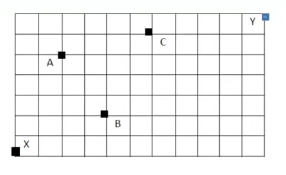
\includegraphics[width=0.3\linewidth]{kraty.png}
    \end{figure}

    \begin{enumerate}[a)]
        \item Przechodzą przez A, B i C?
        \item przechodzą przez A lub B lub C?
        \item Przechodzą przez A lub B, ale nie przechodzą przez C?
    \end{enumerate}
\end{zadanie}
\begin{proof}

    \begin{enumerate}[a)]
        \item Żadna z najkrótszych dróg z X do Y nie przechodzi jednocześnie przez A, B oraz C.
        \item Drogi mogą przechodzić przez A albo B (ale nie jednocześnie przez obydwa), mogą również przechodzić przez A oraz C i B oraz C. Oznacza to że
              liczbę wszystkich dróg można policzyć poprzez zastosowanie wzoru:

              \begin{align*}
                  |A\cup B\cup C| & = |A|+|B|+|C| - |A\cap B| - |A\cap C| - |B\cap C| + |A\cap B\cap C|, \\
                                  & = |A|+|B|+|C|  - |A\cap C| - |B\cap C|.
              \end{align*}

              (ponieważ ustaliliśmy że nie ma dróg $A\cap B$, moc jest zerowa). Liczba wszystkich dróg przechodzących przez A to $\binom72\cdot\binom{11}2$, liczba wszystkich dróg przechodzących przez B to $\binom 62\cdot\binom{11}5$, liczba kroków przez C to $\binom{12}6\cdot\binom61$. Liczba kroków $A\cap C$ to $\binom72\cdot\binom51\cdot\binom61$. Liczba kroków $B\cap C$ to $\binom62\cdot\binom62\cdot\binom61$. Zatem ostateczne równanie to:

              $|A\cup B\cup C| = |A|+|B|+|C|-|A\cap C|-|B\cap C|=\binom72\binom{11}2 + \binom 62\binom{11}5+\binom{12}6\binom61-\binom72\binom51\binom61-\binom62\binom62\binom61.$

        \item Przechodzą przez A lub B, ale nie przechodzą przez C?

              Poszukujemy rozwiązania $|(A\setminus C)\cup (B\setminus C)|$. Ponieważ A oraz B są rozłączne, upraszcza nam to poszukiwania. Od mocy zbioru A musimy odjąć moc zbioru $A\cap C$, od mocy zbioru B musimy odjąć moc zbioru $B\cap C$. Równanie to:

              $|(A\setminus C)\cup (B\setminus C)| = |A| - |A\cap C| + |B| - |B\cap C| = \binom72\cdot\binom{11}2 - \binom72\cdot\binom51\cdot\binom61 + \binom 62\cdot\binom{11}5 -\binom62\cdot\binom62\cdot\binom61.$
    \end{enumerate}
\end{proof}

\begin{zadanie}
    Ile jest najkrótszych dróg z P do K? Uwaga: nie można przechodzić przez pusty obszar wewnątrz kraty.

    \begin{figure}[H]
        \centering
        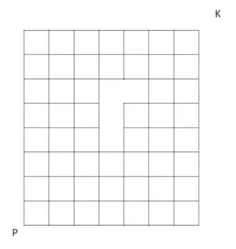
\includegraphics[width=0.3\linewidth]{kraty2.png}
    \end{figure}
\end{zadanie}

\begin{proof}
    Rozwiązanie polega na policzeniu wszystkich najkrótszych dróg z P do K:$\binom{15}7$, po czym odjęciu tych sumy trzech przypadków, gdy przechodzimy przez zakazane "mosty" - nazwijmy je, od dołu, $A, B, C$ (gdzie $C$ jest pionowy). Przejście przez $A$ oraz $B$ się wykluczają, jednak przecięcie obydwu z $C$ jest niepuste. Mamy zatem:
    \begin{itemize}
        \item $|A| = \binom73\binom73$,
        \item $|B| = \binom83\binom63$,
        \item $|C| = \binom94\binom52$,
        \item $|A\cap C| = \binom73\binom52$,
        \item $|B\cap C| = \binom83\binom52$.
    \end{itemize}

    Zbierając do kupy:

    $|A\cup B\cup C| = |A| + |B| + |C| - |A\cap C| - |B\cap C|=\binom73\binom73+\binom83\binom63+\binom94\binom52-\binom73\binom52-\binom83\binom52.$

    A zatem liczba wszystkich rozwiązań to:

    $$\binom{15}7 - \binom73\binom73-\binom83\binom63-\binom94\binom52+\binom73\binom52+\binom83\binom52.$$
\end{proof}


\begin{zadanie}
    (Zmienne są całkowitoliczbowe.)
    Ile rozwiązań ma równanie
    $$x_1 + x_2 + x_3 + x_4 + x_5 + x_6 + x_7 = 40$$
    gdzie $x_1, x_2, x_3$ są dodatnie, $x_4 \geq 5, x_5 > 3, x_6 = 2$,
    $x_7 > 4$.
\end{zadanie}
\begin{proof}
    Stosujemy podstawienie:

    \begin{itemize}
        \item $y_1 = x_1-1$,
        \item $y_2 = x_2-1$,
        \item $y_3 = x_3-1$,
        \item $y_4 = x_4-5$,
        \item $y_5 = x_1-4$,
        \item $y_6 = x_7-5$,
    \end{itemize}
    oraz pozbywamy się $x_6$ z obydwu stron. Uzyskujemy:

    $$y_1+y_2+y_3+y_4+y_5+y_6=21,$$

    gdzie $y_i\geq0$. Liczba rozwiązań to oczywiście $\binom{21+5}{5}$.

\end{proof}

\begin{zadanie}
    Ile (wszystkich) rozwiązań ma nierówność
    $x_1 + x_2 + x_3 \leq 6,$
    gdzie $x_1, x_2, x_3$ są liczbami całkowitymi, nieujemnymi?
\end{zadanie}
\begin{proof}
    Liczba kombinacji to suma przypadków gdy $x_1+x_2+x_3=0,1,2,\dots,6$. Zatem moglibyśmy to rozwiązać poprzez zsumowanie:
    $$\sum_{i=0}6\binom{i+2}{2} = \binom22+\binom32+\binom42+\binom52+\binom62+\binom72+\binom82 = 84.$$
\end{proof}

\begin{zadanie}
    Ile (wszystkich) rozwiązań ma ta nierówność zadania 6., jeśli dodatkowo muszą być spełnione warunki:
    $x_1$ - nieparzysta, $x_2 < 5$,
    $x_3 = 0, 3, 5$? (Tu też zakładamy, że $x_1 , x_2 , x_3$ są liczbami całkowitymi, nieujemnymi)
\end{zadanie}
% \begin{proof}
%     Mamy następujące zbiory przypadków:

%     \item $A$ -
% \end{proof}


\begin{zadanie}
    W sklepie w koszu jest 40 jednakowych skarpet.

    8 (rozróżnialnych) klientów $\{a, b, c, d, e, f, g, h \}$ wybiera je z kosza. Na ile sposobów mogli to zrobić, jeśli:
    \begin{itemize}
        \item każdy klient coś kupił,
        \item każdy kupił parzystą liczbę skarpet,
        \item wszystkie skarpety zostały sprzedane?
    \end{itemize}
\end{zadanie}
\begin{proof}
    Ponieważ każdy klient kupił parzystą liczbę skarpet, możemy podejść do zadania jakbyśmy zliczali 20 jednakowych par skarpet. Dalej, ponieważ każdy z klientów coś kupił, badamy ile par ponad jedną zostało kupione. W końcu, ponieważ wszystkie pary zostały wyprzedane, możemy stworzyć równanie:

    $$x_a+x_b+x_c+x_d+x_e+x_f+x_g+x_h = 20,$$

    lub:

    $$y_a+y_b+y_c+y_d+y_e+y_f+y_g+y_h = 12,$$

    gdzie $y_i = x_i-1$, zatem $y_i\geq 0$. W ten sposób zadanie sprowadzamy do przypadku, gdzie 7 nierozróżnialnych elementów ($n-1$) rozmieszczamy na 12+7 slotach. Mamy zatem $\binom {19}7$ kombinacji.

\end{proof}

\subsection{Zasada Dirichleta - zastosowanie}
Przytoczę tutaj \textit{zasadę szufladkową Dirichleta}:

\begin{theorem}[Zasada szufladkowa Dirichleta]
    Jeśli $X$ oraz $Y$ są niepustymi zbiorami skończonymi i $f\in Fun(X,Y)$ oraz
    $|X| > r\cdot |Y|$ dla pewnego $r>0$, to co najmniej jeden ze zbiorów $f^{-1}(\{y\})$ ma więcej niż $r$ elementów.
\end{theorem}
\begin{proof}
    Istotnie, jeśli maksimum elementów w $|Y|$ zbiorach to $r$, to nie możemy mieć więcej niż $|Y|\cdot r$ elementów we wszystkich zbiorach. Zatem $|X| >r\cdot|Y|$ gwarantuje nam istnienie przynajmniej jednego zbioru o przynajmniej $r+1$ elementach.
\end{proof}


\begin{zadanie}
    W cukierni jest 8 różnych smaków lodów. Deser = kubek z 5 różnymi gałkami lodów. Było 120 klientów. Czy to prawda, że co najmniej 3 klientów wybrało taki sam deser?
\end{zadanie}
\begin{proof}
    Możliwych do wybrania deserów jest $\binom85 = 56$. Jeśli maksymalną liczbą klientów którzy wybrali ten sam deser byłoby dwa, oznacza to że nie mogło być więcej niż 112 klientów. Ponieważ mieliśmy 120 klientów, istniał przynajmniej jeden taki deser który został wybrany przez 3 lub więcej klientów.
\end{proof}


\begin{zadanie}
    83 pomarańcze umieszczono w 9 koszach.
    \begin{enumerate}[a)]
        \item Czy to prawda, że musi istnieć przynajmniej jeden kosz, do którego trafiło 20 pomarańczy?
        \item Czy to prawda, że musi istnieć przynajmniej jeden kosz, do którego trafiło więcej niż 9 pomarańczy?
    \end{enumerate}
\end{zadanie}
\begin{proof}
    \begin{enumerate}[a)]
        \item Kontrprzykład - rozkładamy pomarańcze po 9 do każdego kosza i 11 do ostatniego.
        \item W tym wypadku $83 > 9\cdot 9$, zatem musi istnieć kosz do którego trafiło przynajmniej 10 pomarańczy.
    \end{enumerate}
\end{proof}

\begin{zadanie}
    10 drużyn rozegrało 8 meczów. Udowodnić, że są przynajmniej dwie drużyny, które rozegrały tyle samo spotkań.
\end{zadanie}
\begin{proof}
    Każda z 10 drużyn mogła rozegrać co najwyżej 8 meczów. Jeśli byśmy przyporządkowywali każdej z drużyn liczbę meczów, to przynajmniej jedna z liczb meczów musiałaby mieć wiecej niż jedną drużynę.
\end{proof}


\begin{zadanie}
    X = zbiór ciągów binarnych długości 10. Czy w X musi istnieć 80 ciągów, których suma wyrazów jest taka sama?
\end{zadanie}
\begin{proof}
    Wszystkich możliwych ciągów binarnych jest $1024$ ($2^{10}$). Wszystkich możliwych wartości ciągów jest 9 (od 0 do 8). Jeśli nie istniałoby 80 ciągów o tej samej wartości, wtedy maksymalną możliwą liczbą ciągów o tej samej wartości byłoby 79 - oznaczałoby to co najwyżej $9\cdot79=711$ możliwych ciągów. Stąd zatem wiemy, że musi istnieć przynajmniej 80 ciągów o tej samej wartości.
\end{proof}




\subsection{Zliczanie podzbiorów}

% \begin{zadanie}
%     Wykonaj mnożenie poniższych trzech wielomianów:
%     $$[ ( x_1 + x_3 + x_5 + x_7 )\cdot ( x_1 + x_2 + x_4 ) ] \cdot ( x_1 + x_2 ).$$
% \end{zadanie}
% \begin{proof}
% \end{proof}
% \begin{zadanie}
%     $X = \{7a, 4b, 2c\}$; rozważ takie podzbiory, w których element a występuje nieparzystą liczbę razy, zaś
%     elementy b i c występują parzystą liczbę razy. Skonstruuj funkcję tworzącą dla ciągu liczb podzbiorów
%     k-elementowych, spełniających podany warunek. Ile takich podzbiorów zawiera więcej niż 5 elementów?
% \end{zadanie}
% \begin{proof}
% \end{proof}

\begin{zadanie}
    \begin{enumerate}[a)]
        \item Jest 8 osób. Trzeba utworzyć 3 rozłączne grupy, liczące odpowiednio $2$, $3$ i $3$ osoby. Na ile sposobów można to zrobić?
        \item Mamy cyfry $7,7,5,5,5,2,2,2$. Ile ośmiocyfrowych liczb można utworzyć, zapisując w dowolnej kolejności te cyfry?
    \end{enumerate}
\end{zadanie}

\begin{proof}
    Zadanie rozwiązujemy w obydwu przypadkach poprzez iloczyn trzech symboli Newtona:

    $$\binom 82\cdot\binom 63\cdot\binom 33.$$

    W drugim przypadku tworzymy trzy zbiory z ośmiu elementów pozycji cyfr od 1 do 8 - dwuelementowy zbiór pozycji na których jest cyfra $7$, trójelementowy zbiór pozycji cyfr $5$ oraz trójelementowy zbiór pozycji cyfr $2$.
\end{proof}
\begin{zadanie}
    Dany jest zbiór z powtórzeniami:

    $$X = \{3a, 2b, 4c\}.$$

    \begin{enumerate}[a)]
        \item Ile elementów ma X?
        \item Ile podzbiorów ma X (chodzi o podzbiory z powtórzeniami)?
    \end{enumerate}
\end{zadanie}
\begin{proof}
    \begin{enumerate}[a)]
        \item Ile elementów ma X?

              Odpowiedź to 9: suma krotności wszystkich elementów.

        \item Ile podzbiorów ma X (chodzi o podzbiory z powtórzeniami)?

              Odpowiedź: $4\cdot3\cdot5$ (wszystkie kombinacje 0-3 elementy $a$, 0-2 elementy $b$, 0-4 elementy $c$).
    \end{enumerate}
\end{proof}

\subsection{Funkcje tworzące}
\begin{zadanie}
    Dany jest zbiór z powtórzeniami: $X=\{7a, 4b, 2c\}$. Rozważ takie podzbiory, w których element $a$ występuje nieparzystą liczbę razy, zaś elementy $b$ i $c$ występują parzystą liczbę razy.

    Ile takich podzbiorów zawiera więcej niż 5 elementów?
\end{zadanie}

\begin{proof}
    Rozważamy przypadki kiedy mamy $1,3,5,7$ elementy $a$, $0,2,4$ elementy $b$ oraz $0,2$ elementy $c$. Daje to nam $4\cdot 3\cdot2 = 24$ możliwości.

    Aby policzyć liczbę podzbiorów o więcej niż 5 elementach, użyjemy następującego algorytmu postępowania:

    \begin{itemize}
        \item Zareprezentujemy każdą z liczb elementów (tj. 1,3,5,7 elementów $a$ itd.) jako sumę potęg $x$. Następnie przemnożymy przez siebie powstałe w ten sposób wielomiany.
        \item Powstanie wielomian, w którym potęgi przy $x$ będą reprezentowały liczbę elementów, natomiast liczby przy tych potęgach - liczby możliwości. Należy zliczyć i dodać wszystkie interesujące nas możliwości.
    \end{itemize}

    W tym wypadku mamy następujące wyrażenie:

    $$(x^1+x^3+x^5+x^7)\cdot(x^0+x^2+x^4)\cdot(x^0+x^2) =x^{13} + 3 x^{11} + 5 x^9 + 6 x^7 + 5 x^5 + 3 x^3 + x^1 ,$$
    czyli mamy: 1 kombinację zbioru o 13 elementach, 3 kombinacje zbiorów o 11 elementach, 5 kombinacji zbiorów o 9 elementach... itd. Zatem zbiorów które mają więcej niż 5 elementów będzie $1+3+5+6 = 15.$
\end{proof}

\begin{zadanie}
    $A=\{1,2,3,4,5,6,7,8,9\}$. Rozpatrujemy tylko liczby sześciocyfrowe, utworzone z cyfr ze zbioru A. Ile jest liczb, w których występują przynajmniej trzy cyfry 5?
\end{zadanie}

\begin{proof}
    Zbiór wszystkich liczb sześciocyfrowych złożonych z elementów $A$ ma $9^6$ kombinacji. Jeśli chcemy teraz policzyć wszystkie kombinacje, w których są przynajmniej trzy cyfry $5$, to musimy odjąć wszystkie:
    \begin{itemize}
        \item kombinacje w których są dokładnie 2 cyfry 5: $\binom 62\cdot8^4$ (nierozróżnialne piątki w 2 z 6 miejsc, 8 możliwych cyfr na 4 pozostałych miejscach)
        \item kombinacje w których jest dokładnie 1 cyfra 5: $\binom 61\cdot8^5$ (piątka w 1 z 6 miejsc, 8 możliwych cyfr na 5 pozostałych miejscach)
        \item kombinacje w których nie ma cyfry 5: $8^6$ (8 możliwych cyfr na 6 pozycjach).
    \end{itemize}

    Liczba wszystkich kombinacji:

    $$9^6 - \binom 62\cdot8^4-\binom 61\cdot8^5-\cdot8^6.$$

\end{proof}

\begin{zadanie}
    Cyfry $\{ 1, 2, 3, 4, 5 \}$, litery $\{ a, b, c, d, e, f \}$. Ile różnych ciągów długości 7 można utworzyć, jeśli na dwóch ostatnich
    pozycjach nie mogą wystąpić te same litery? Ile jest ciągów, w których występują najwyżej cztery litery?
\end{zadanie}

\begin{zadanie}
    Tworzymy kody długości 10 z dwóch znaków b oraz c. Ile jest kodów, które mają nie więcej niż 5 znaków b?
\end{zadanie}

\begin{zadanie}
    Dziesięć osób $\{ o_1,\dots,o_{10} \}$ przydzielono do trzech zespołów $\{ z_1, z_2, z_3 \}$. Ile jest sposobów przydziału, jeśli do każdego zespołu ktoś trafił?
\end{zadanie}

\begin{zadanie}
    Ile jest permutacji zbioru $\{1, 2, \dots, 10\}$, takich że 2 i 7 lub 6 i 8 stoją obok siebie?
\end{zadanie}
\begin{proof}
    Należy policzyć wszystkie możliwe permutacje i odjąć od nich sumę zbiorów w których stoją obok siebie 2 i 7 lub 6 i 8. Zatem:

    \begin{itemize}
        \item Wszystkich ciągów jest $10!$,
        \item ciągów w których 2 i 7 stoją obok siebie jest $9\cdot 2!\cdot 8!$,
        \item identycznie z ciągami gdzie 6 i 8 stoją obok siebie,
        \item ciągi w których 2 i 7 oraz 6 i 8 stoją obok siebie - mamy dwie kombinacje - najpierw 2 i 7, potem 6 i 8, lub odwrotnie. Każda z nich ma dwie kombinacje kolejności 2 i 7, oraz dwie kombinacje 6 i 8. Pozostaje zliczyć na ile sposobów możemy rozmieścić dwie pary na 10 pozycjach:
              \begin{itemize}
                  \item Jeśli pierwsza para jest na miejscu 1, to drugą można wstawić na 7 miejscach (8-1).
                  \item Jeśli pierwsza para jest na miejscu 2, to drugą można wstawić na 6 mijescach (7-1),
                  \item \dots
                  \item itd.
              \end{itemize}

              Zatem mamy $7+6+\dots+2+1 = 8\cdot7/2 = 28$ możliwości postawienia par. Daje nam to w sumie $2\cdot2\cdot2\cdot28 = 224$ kombinacje.

    \end{itemize}

    Chcemy zatem policzyć wszystkie możliwe kombinacje z uwzględnionymi warunkami:

    $$|\Omega\setminus(A\cup B)| = |\Omega| - |A\cup B| = |\Omega| - (|A|+|B|-|A\cap B|) = 10! - (9\cdot2!\cdot8! +9\cdot2!\cdot8!-224).$$
\end{proof}

\begin{zadanie}
    Mamy ciągi długości 12, o wyrazach z $\{ a, b, c, d, e, f, g \}$.
    \begin{enumerate}[a)]
        \item Ile jest ciągów, w których nie ma znaków b lub c lub d?
        \item Ile jest ciągów, w których jest przynajmniej jedna b-tka i przynajmniej jedna c-tka?
    \end{enumerate}
\end{zadanie}
\begin{proof}
    \begin{enumerate}[a)]
        \item Ile jest ciągów, w których nie ma znaków b lub c lub d?

              Zliczamy moce zbiorów ciągów 12-znakowych które nie zawierają liter:
              \begin{itemize}
                  \item $|b| = |c| = |d| = 7^{12}$,
                  \item $|b\cap c| =|c\cap d| =|d\cap b| = 6^{12}$,
                  \item $|b\cap c\cap d| = 5^{12}$,
              \end{itemize}

              Korzystamy z zasady wyłączania zbiorów:

              $$|b\cup c\cup d| = |b|+|c|+|d| - |b\cap c| - |c\cap d|-|b\cap d| + |b\cap c\cap d|=3\cdot7^{12}-3\cdot 6^{12}+5^{12}.$$

        \item Ile jest ciągów, w których jest przynajmniej jedna b-tka i przynajmniej jedna c-tka?

              Najprościej rozwiązać zadanie poprzez znalezienie różnicy zbioru wszystkich rozwiazań oraz sumy zbiorów gdzie jest przynajmniej jeden z elementów. Mamy zatem:

              \begin{itemize}
                  \item $|\Omega| = 7^{12}$,
                  \item $|B| = 12\cdot 6^{11}$,
                  \item $|C| = 12\cdot 6^{11}$,
                  \item $|B\cap C| = 12\cdot11\cdot2\cdot 5^{10}$,
              \end{itemize}

              zatem całkowita liczba zbiorów gdzie mamy przynajmniej jedną b-tkę i c-tkę to:

              $$|\Omega\setminus(B\cup C)| = |\Omega|-|B\cup C| = |\Omega| - (|B|+|C|-|B\cap C|) = 7^{12} - (12\cdot 6^{11}+12\cdot 6^{11}-12\cdot11\cdot2\cdot 5^{10}).$$

    \end{enumerate}
\end{proof}

\end{document}